\section{Introduction}
\label{sec:introduction}
Consider the problem of reconstructing a 3D shape from silhouettes. 
The classic visual hull algorithm that intersects the visible volumes
from each viewpoint is easy to implement but is sensitive to errors in
viewpoint estimation and silhouette noise.
A Bayesian approach for this problem would be to add appropriate
priors over the shape and viewpoint estimates and perform posterior
inference.
This is challenging for two reasons. First, the search space of 3D
shape is large since there is no compact shape basis to search
over for general shapes.
Second, Bayesian inference is typically expensive for high-dimensional data.

To this end we present \emph{differentiable projection operators}
$\cal{T}$ and \emph{deep shape priors} for which Bayesian inference
can be performed via stochastic gradient descent and their
variants~\cite{sgld}.
While many priors exist, of interest is the ``deep shape prior"
of Ulyanov \etal~\cite{ulyanov17deep} which showed that the space of
natural images $\bm{x}$ can represented as a parametric family
$f_{\bm{\theta}}(\eta)$ where $f$ is a convolutional network, $\theta$
its parameters, and $\eta$ is a fixed input. Their work showed that
search over natural images can be replaced by a search over the
parameters of the network $\bm{\theta}$, which can be efficiently done
via gradient descent.

\begin{figure}
\centering
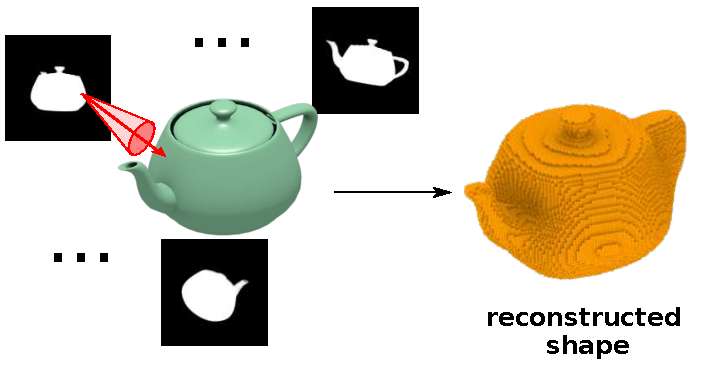
\includegraphics[width=0.6\linewidth]{dsp/figs/splash.pdf}
\caption{\label{fig:splash}\small
\textbf{Shape reconstruction from binary images with uncertain viewpoints.}
    We propose to use deep networks together with differentiable projection operators for shape reconstruction.
    Our approach leverages the shape prior induced by neural networks to reconstruct shapes from projections
    without any learning procedure.
    Additionally, our approach can use differentiable operators to reconstruct shapes under noisy projection
    measurements, like perturbed viewpoint information.}
\vspace{-12pt}
\end{figure}


Our work takes this idea further. First, we endow the deep image prior
with 3D convolutions resulting in a deep shape prior.
Second, we incorporate differentiable projection operators ${\cal T}$ that model
projection measurements, such as silhouettes, given projection
parameters $\phi$ such as viewpoints.
Thus inferring a shape $\bm{x}$ given noisy projection measurements
$\bm{y}$ reduces to the following optimization over network parameters
$\bm{\theta}$ and projection parameters $\phi$:
\begin{equation}
\label{eq:maineq}
	\min_{\phi, \bm{\theta} \in \mathbb{R}^D} E\left(\bm{y}, {\cal T}(f_{\bm{\theta}}(\bm{\eta}), \phi)\right) + P(\phi), 
\end{equation}
where $P(\phi)$ is a prior over projection parameters, which is often
a simple function. We show that for a number of shape construction
problems such as tomographic reconstruction, shape from silhouettes or
depth maps, it is possible to construct projection operators using
existing neural network building blocks that are differentiable with
respect to both the input and projection parameters.
Thus the objective can be minimized using ``backpropagation" machinery, 
which is generally much faster than Bayesian inference using Markov
Chain Monte Carlo (MCMC) techniques.




Apart from choosing the network architecture and the projection
operator, the approach does not require any task-specific training.
Nevertheless, it yields compelling results for tomographic
reconstruction in the low sampling regime, where it outperforms a
state-of-the-art approach based on iterative
BM3D~\cite{maggioni2013nonlocal}.
Our work also shows that the deep image prior generalized to 3D
volumes is effective at modeling 3D shapes.
In problems such as visual hull reconstructions, or reconstruction from
depth maps, we can accurately estimate the 3D shape of an object from
only a few views, even when there are uncertainties in the view
estimates, or when depth maps are corrupted by noise.
The reconstruction results are significantly better than handcrafted priors.
These tasks are illustrated in Figures~\ref{fig:ct}-\ref{fig:depthview}.
